\documentclass[a4paper, 12pt]{article}

\usepackage[utf8]{inputenc}
\usepackage[document]{ragged2e}
\usepackage{graphicx}
\usepackage{tikz}
\usepackage{multicol}
\usepackage{multirow}
\usepackage{hyperref}
\usepackage{tabu}
\usepackage{booktabs}
\usepackage{vwcol}
\usepackage[inline]{enumitem}

\usepackage[left=20pt, top=20pt, right=20pt]{geometry}

\graphicspath{{./img/}}
\hypersetup{
    colorlinks=true,
    linkcolor=blue,
    filecolor=magenta,      
    urlcolor=cyan,
}

\urlstyle{same}

\begin{document}

\begin{vwcol}[widths={0.2, 0.8}]
  \begin{tikzpicture}
    \clip (0,0) circle(1.5cm);
    \node[anchor=center] at (0,0) {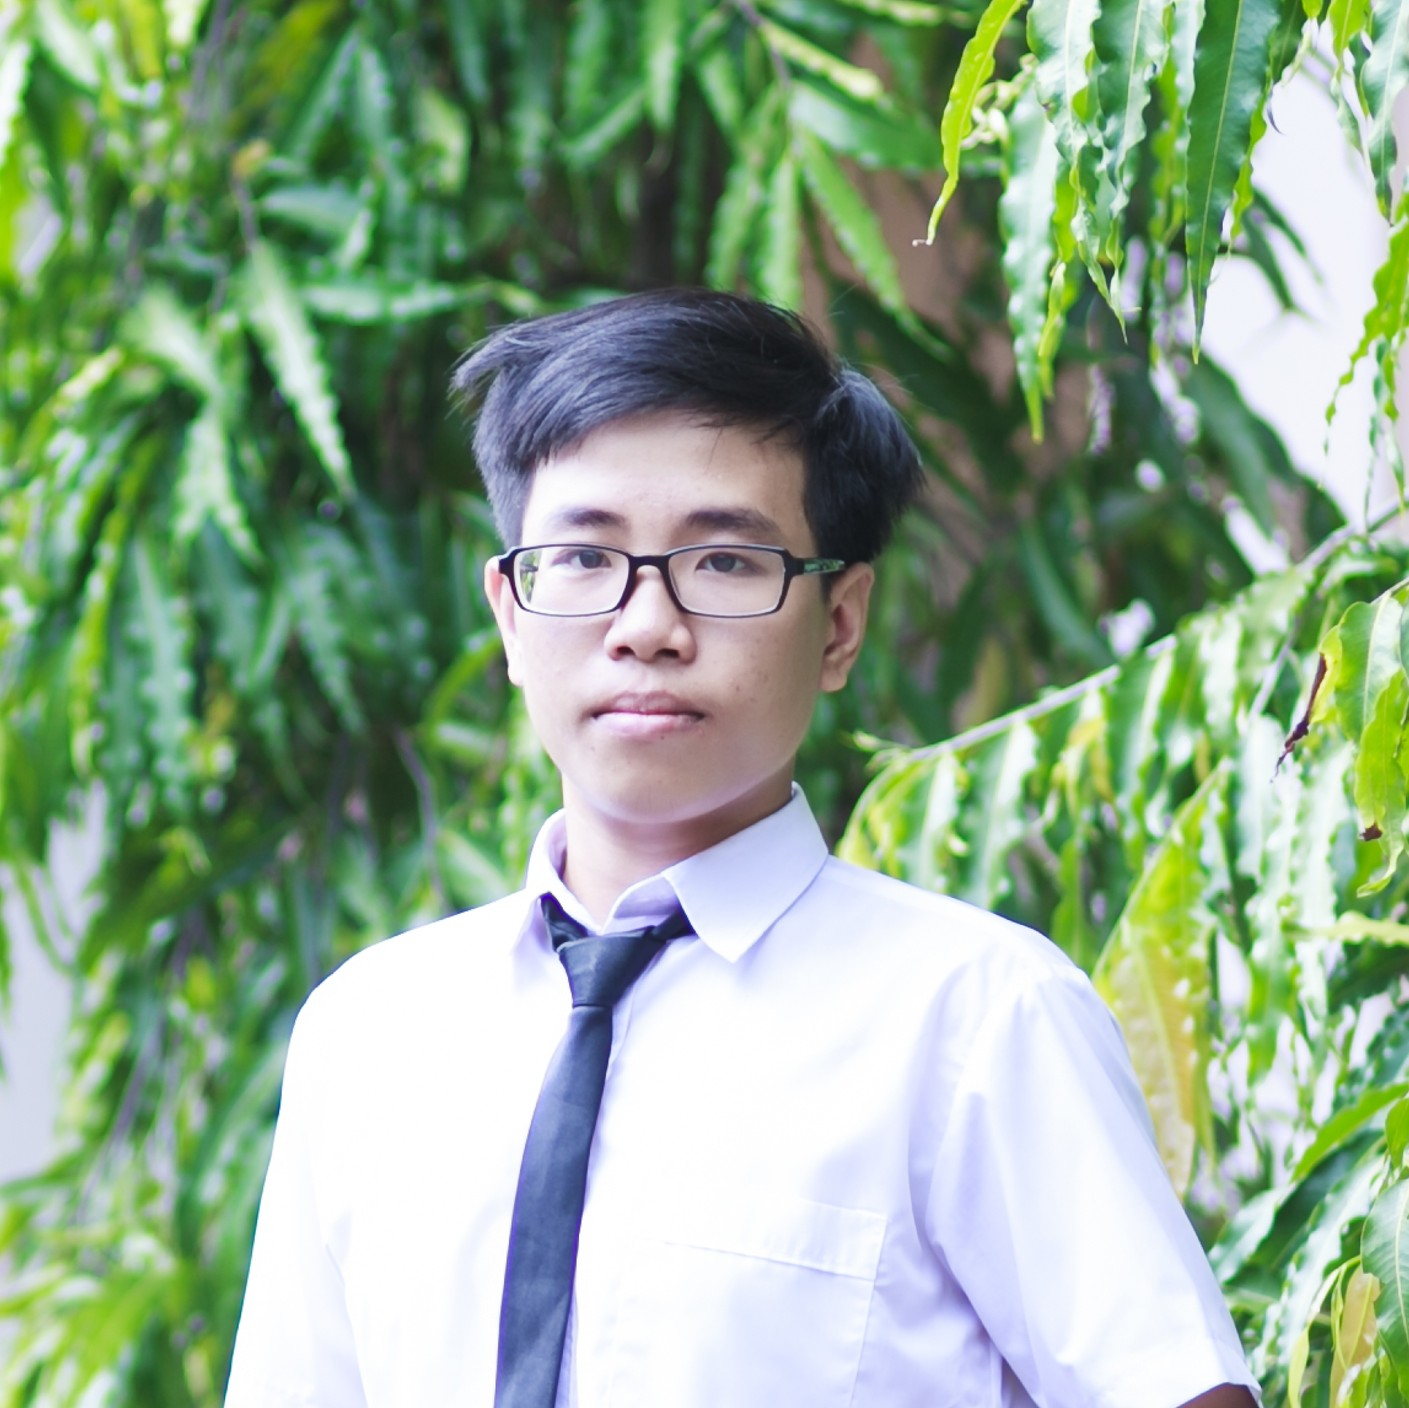
\includegraphics[width=3cm]{ava}};
  \end{tikzpicture}

  \hspace{0pt}
  \vfill
  \begin{tabular}{l|l}
    \multicolumn{2}{l}{\Huge{\textbf{\textcolor[rgb]{0.5,0.8,0.4}{Tuan-Dat Le}}}}
    \vspace{5mm}\\
    Email: letuandat2110@gmail.com & Phone: 0941623569 \\
    \url{github.com/ledat2110} & \url{linkedin.com/in/ledat2110}
  \end{tabular}
  \vfill
  \hspace{0pt}
\end{vwcol}

\line(1,0){550}\\
Computer scientist looking for a position at a R\&D lab, where I can apply my knowledge about Computer vision, Reinforcement learning to support internal and external communication \\

\line(1,0){550}\\
\vspace{3mm}
{\huge Education}
\begin{itemize}
    \item VNUHCM - University of Science
    \item BCs in Computer Science, Honor program
    \item GPA: 8.5/10
\end{itemize}

\line(1,0){550}\\
\vspace{3mm}
{\huge Skills}
\begin{itemize}
    \item Programming languages: Python, C++
    \item Framework: PyTorch
    \item Research: Computer vision, Reinforcement learning
    \item Soft skills: Critical thinking, Creativity, Emotional intelligence, Adoptability
\end{itemize}

\line(1,0){550}\\
\vspace{3mm}
{\huge Projects}
\begin{itemize}
    \item Cart-pole Game | Leader | 20/08/2020 - 20/9/2020
      \begin{itemize}
          \item Cartpole - known also as an Inverted Pendulum is a pendulum with a center of gravity above its pivot point. It’s unstable, but can be controlled by moving the pivot point under the center of mass. The goal is to keep the cartpole balanced by applying appropriate forces to a pivot point.
          \item Team size: 1 member
          \item Responsibility:
            \begin{itemize}
                \item Creating an agent that is capable of learning through trial and error and ultimately solving the cartpole problem.
            \end{itemize}
          \item Tech stacks:
            \begin{itemize}
                \item Deep Q-learning
                \item Deep Neural Network
                \item Buffer replay in DQN
            \end{itemize}
        \end{itemize}
    \item AIC HCMC | Member | 10/07/2020 - 05/09/2020
      \begin {itemize}
      \item There are four types of vehicles in the road. In this project, the mission is counting the exact number of each type vehicles moving in the specific direction.
      \item Team size: 5 members
      \item Responsibility:
        \begin{itemize}
          \item Labeling the objects in videos of the dataset.
          \item Training model to detect the vehicles occuring in the videos
        \end{itemize}
      \item Tech stacks: 
        \begin{itemize}
          \item Using YOLOv4 model to detect the vehicles appearing in the videos.
          \item Using LabelImg to label the vehicles in the dataset.
        \end{itemize}
      \end{itemize}

    \item Self-drving Car | Leader | 20/01/2020 - 28/04/2020
      \begin {itemize}
        \item There is a car equiped with 5 ultra-sonic sensors to measure the distance between the car and walls on two side of road. The mission is making the car autonomously run to the destination.
        \item Team size: 2 member
        \item Responsibility:
        \begin{itemize}
          \item Determinig the algorithm and model used to solve the problem
          \item Building the neural network
          \item Tuning the hyperparametes so that the weights of the model can converge
        \end{itemize}
        \item Tech stacks: 
        \begin{itemize}
          \item Using genetic algorithm to optimize the weights of the model
          \item Using a neural network with 3 fully connected layers.
        \end{itemize}
        \item Link: \url{github.com/ledat2110/Self-driving-Car-using-Neural-Network}
      \end{itemize}

    \item Image classification | Leader | 15/01/2020 - 20/03/2020
      \begin{itemize}
        \item This is a school project. The mission is building a model to classify the class of the image in the dataset. Each image contains an object with specific class. There are 10 classes at all.
        \item Team size: 1 member
        \item Responsibility:
          \begin{itemize}
              \item Building a CNNs, which is capable of classifying the objects with the accuracy above 95\%.
          \end{itemize}
        \item Tech stacks:
          \begin{itemize}
              \item Convolutional neral network
          \end{itemize}
        \item Link: \url{github.com/ledat2110/cs231n}
      \end{itemize}

      
\end{itemize}

\line(1,0){550}\\
\vspace{5mm}
{\huge Achivement}
\begin{itemize}
    \item Top 35 | AIC HCMC 2020
    \item Top 27 | VNUHCM - University of Science Challenge 2020
    \item Top 27 | VNUHCM - University of Science Challenge 2019
\end{itemize}
\end{document}
